\documentclass[a4paper,14pt]{extreport} % формат документа

\usepackage{amsmath}
\usepackage{cmap} % поиск в ПДФ
\usepackage[T2A]{fontenc} % кодировка
\usepackage[utf8]{inputenc} % кодировка исходного текста
\usepackage[english,russian]{babel} % локализация и переносы
\usepackage[left = 2cm, right = 1cm, top = 2cm, bottom = 2 cm]{geometry} % поля
\usepackage{listings}
\usepackage{graphicx} % для вставки рисунков
\usepackage{amsmath}
\usepackage{float}
\usepackage{multirow}
\graphicspath{{pictures/}}
\DeclareGraphicsExtensions{.pdf,.png,.jpg}
\newcommand{\anonsection}[1]{\section*{#1}\addcontentsline{toc}{section}{#1}}

\lstset{ %
	language=Lisp,                % Язык программирования 
	numbers=left,                   % С какой стороны нумеровать          
	frame=single,                    % Добавить рамку
}

\begin{document}
\begin{titlepage}

    \begin{table}[H]
        \centering
        \footnotesize
        \begin{tabular}{cc}
            \multirow{8}{*}{
\includegraphics[scale=0.35]{bmstu.jpg}}
            & \\
            & \\
            & \textbf{Министерство науки и высшего образования Российской Федерации} \\
            & \textbf{Федеральное государственное бюджетное образовательное учреждение} \\
            & \textbf{высшего образования} \\
            & \textbf{<<Московский государственный технический} \\
            & \textbf{университет имени Н.Э. Баумана>>} \\
            & \textbf{(МГТУ им. Н.Э. Баумана)} \\
        \end{tabular}
    \end{table}

    \vspace{-2.5cm}

    \begin{flushleft}
        \rule[-1cm]{\textwidth}{3pt}
        \rule{\textwidth}{1pt}
    \end{flushleft}

    \begin{flushleft}
        \small
        ФАКУЛЬТЕТ
        \underline{<<Информатика и системы управления>>\ \ \ \ \ \ \ 
        \ \ \ \ \ \ \ \ \ \ \ \ \ \ \ \ \ \ \ \ \ \ \ \ \ \ \ \ \ \ \ 
    \ \ \ \ \ \ \ \ \ \ \ \ \ \ \ } \\
        КАФЕДРА
        \underline{<<Программное обеспечение ЭВМ и
        информационные технологии>>
        \ \ \ \ \ \ \ \ \ \ \ \ \ \ \ \ \ \ \ \ }
    \end{flushleft}

    \vspace{2cm}

    \begin{center}
        \textbf{Лабораторная работа № 4} \\
        \vspace{0.5cm}
    \end{center}

    \vspace{4cm}

    \begin{flushleft}
        \begin{tabular}{ll}
            \textbf{Дисциплина} & Моделирование.  \\
            \textbf{Тема} & Моделирование системы.  \\
            \\
            \textbf{Студент} & Сиденко А.Г. \\
            \textbf{Группа} & ИУ7-73Б \\
            \textbf{Оценка (баллы)} & \\
            \textbf{Преподаватель} & Рудаков И.В.   \\
        \end{tabular}
    \end{flushleft}

    \vspace{4cm}

   \begin{center}
        Москва, 2020 г.
    \end{center}

\end{titlepage}

\begin{enumerate}

\item \textbf{Условие. }

Необходимо промоделировать систему, состоящую из генератора, памяти и обслуживающего аппарата. 

Генератор выдает сообщение распределенные по равномерному закону, они приходят в память и обрабатываются по нормальному закону, параметры задаются. 

Необходимо определить оптимальную длину очереди, при которой не будет потерянных сообщений. Используя принципы $\Delta t$ и событий. 

Как только определили выходной поток сообщений, задаваемую часть сообщений A снова подаем в очередь.

\item \textbf{Теория. }

\textbf{Принцип $\Delta t$:}

\begin{itemize}
\item Ввод данных. 
\item Установка времени в 0. 
\item Получение времени обработки и генерации.  
\item Цикл, пока количество заявок меньше обработанных. 
\begin{itemize}
\item Если время генерации меньше текущего, пришла новая заявка. 
\item Если время обработки меньше текущего, обработка заявки завершена, следующая заявка поступает на обработку. 
\item Увеличение текущего времени на $\Delta t$. 
\end{itemize}
\item Вывод полученных результатов. 
\end{itemize}

\textbf{Событийный принцип:}

\begin{itemize}
\item Ввод данных. 
\item Получение времени обработки и генерации.  
\item Цикл, пока количество заявок меньше обработанных. 
\begin{itemize}
\item Определяется наиболее раннее событие. 
\item В зависимости от события, выполняем действия: пришла новая заявка, либо обработка заявки завершена, следующая заявка поступает на обработку. 
\end{itemize}
\item Вывод полученных результатов. 
\end{itemize}

\item \textbf{Полученные результаты. }

Ниже представлены результаты для различного числа вовзращаемых заявок. 

$$a=1$$
$$b=10$$
$$\mu=0$$
$$\sigma=1$$
$$n=1000$$

Для метода $\Delta t$:
$$\Delta t=1$$

Пример 1 -- $p=0\%$.  
\begin{figure}[H]
  \centering
  \caption{Пример 1. }
  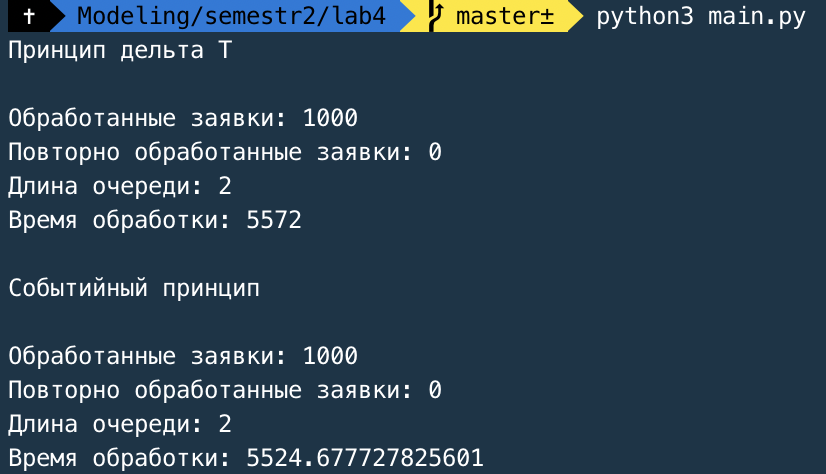
\includegraphics[scale=0.7]{1}
\end{figure}

Пример 2 -- $p=20\%$.  
\begin{figure}[H]
  \centering
  \caption{Пример 2. }
  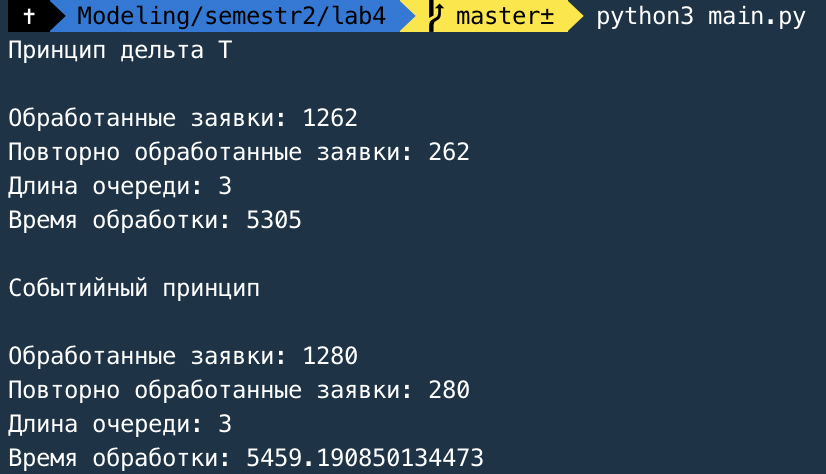
\includegraphics[scale=0.7]{2}
\end{figure}

\newpage

Пример 3 -- $p=50\%$.  
\begin{figure}[H]
  \centering
  \caption{Пример 3. }
  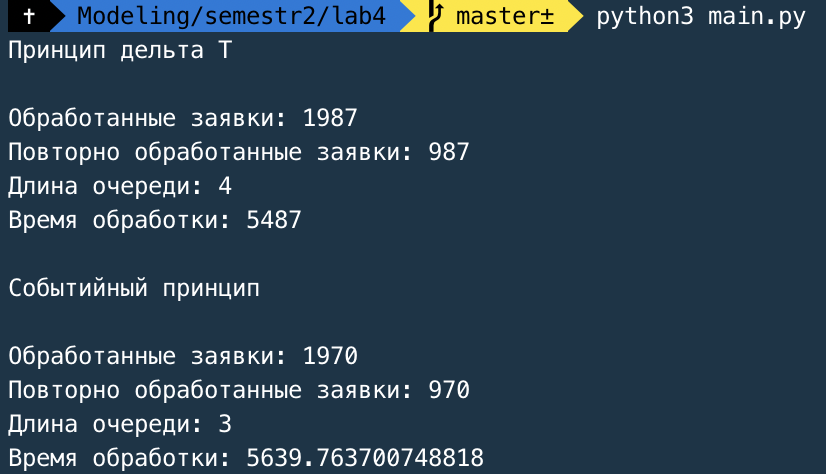
\includegraphics[scale=0.7]{3}
\end{figure}

Пример 4 -- $p=80\%$.  
\begin{figure}[H]
  \centering
  \caption{Пример 4. }
  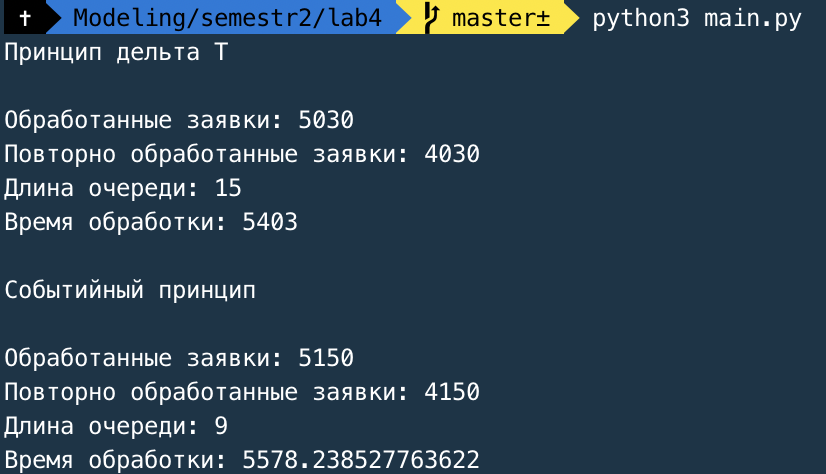
\includegraphics[scale=0.7]{4}
\end{figure}

Пример 5 -- $p=99\%$.  
\begin{figure}[H]
  \centering
  \caption{Пример 5. }
  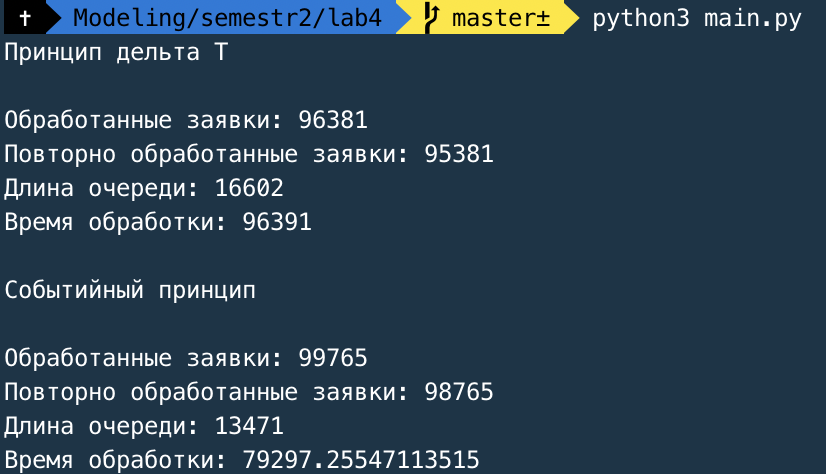
\includegraphics[scale=0.7]{5}
\end{figure}

\item \textbf{Вывод. }

Была смоделирована система, состоящая из генератора, памяти и обслуживающего аппарата. 

На выходе получаем оптимальную длину очереди, число обработанных и повторно обработанных заявок, время обработки. 

\end{enumerate}


\end{document}